\documentclass[11pt,a4paper]{article}
\usepackage[spanish,es-tabla]{babel}
\usepackage[utf8]{inputenc}
\usepackage[T1]{fontenc}
\usepackage{lmodern}
\usepackage[margin=2.2cm]{geometry}
\usepackage{graphicx,booktabs,multirow,float,amsmath,amssymb,listings,xcolor,hyperref}
\usepackage{caption}
\captionsetup{font=small,labelfont=bf}
\graphicspath{{figs/}}
\lstset{basicstyle=\ttfamily\footnotesize,frame=single,breaklines=true,
        keywordstyle=\color{blue!60!black},commentstyle=\color{gray}}

% Etiquetas de los computadores (deben coincidir con las carpetas de results/)
\newcommand{\pcA}{pc1-mac}
\newcommand{\pcB}{pc2-ubuntu}

% Notas del borrador: borrar \nota{...} al redactar la version final.
\newcommand{\nota}[1]{\par\noindent\colorbox{yellow!25}{\parbox{\dimexpr\linewidth-2\fboxsep}{\small\textbf{Borrador:} #1}}\par}

\title{Tarea 2: Multiplicación de matrices con OpenMP y Numba\\
\large IIC3533 Computación de Alto Rendimiento · 2026-2}
\author{Integrante 1 \and Integrante 2 \and Integrante 3}
\date{16 de octubre de 2026}

\begin{document}
\maketitle

% ======================================================================
\section{Introducción}
\nota{Contexto: $C=A\cdot B$ densa de $N\times N$ con costo $O(N^3)$ ($2N^3$ FLOP). Se estudian tres versiones paralelas: (1) paralelismo de datos con OpenMP, (2) dividir y conquistar con tareas OpenMP y (3) Numba. Objetivo: medir el tiempo, el speedup y la eficiencia, y estudiar el efecto del tamaño de bloque, del tamaño del problema y del hardware.}

% ======================================================================
\section{Metodología}
\subsection{Computadores}
\begin{table}[H]
\centering\small
\caption{Características de los computadores usados.}
\label{tab:maquinas}
\begin{tabular}{lll}
\toprule
 & \textbf{PC1 (\pcA)} & \textbf{PC2 (\pcB)} \\
\midrule
CPU & Apple M5 (ARM64) & AMD Ryzen 5 3600X (x86-64, Zen 2) \\
Cores físicos & 10 (4 P-cores + 6 E-cores) & 6 (homogéneos) \\
Cores lógicos & 10 (sin SMT) & 12 (SMT, 2 hilos/core) \\
Frecuencia de reloj & \textbf{COMPLETAR} GHz (P-cores, máx.) & 3.8 GHz base / 4.4 GHz boost \\
Caché L1d & 128 KB/P-core, 64 KB/E-core & 32 KB/core \\
Caché L2 & 16 MB (clúster P) + 6 MB (clúster E) & 512 KB/core \\
Caché L3 & -- & 16 MB (según \texttt{lscpu}) \\
Memoria & 16 GB LPDDR5X unificada & 12 GB visibles en WSL2 (DDR4) \\
Sistema operativo & macOS 26 (Darwin 25.6) & Ubuntu 24.04 sobre WSL2 (Windows) \\
Compilador C++ & Apple clang 21 + libomp & g++ 13.3 (libgomp) \\
Python / Numba & 3.12 / 0.68 & 3.14 / 0.68 \\
\bottomrule
\end{tabular}
\end{table}
\nota{Completar la frecuencia del M5: macOS no la expone por \texttt{sysctl}, así que hay que tomarla de la especificación de Apple. La L1d del Ryzen aparece en \texttt{lscpu} como 192 KiB en 6 instancias, es decir, 32 KB por core. El PC2 corre Ubuntu dentro de WSL2 (máquina virtual de Windows), lo que puede agregar algo de ruido y hace que el scheduler de Windows decida la ubicación final de los threads.}

\subsection{Compilación, medición y verificación}
\begin{itemize}
  \item C++ compilado con \texttt{-O3 -march=native -fopenmp}. En macOS (Apple clang, ARM) el equivalente es \texttt{-O3 -mcpu=native -Xpreprocessor -fopenmp -lomp} con \texttt{libomp} de Homebrew. En Ubuntu se usa \texttt{g++}.
  \item Las matrices se inicializan de forma determinista (igual que \texttt{serial.cpp}): $A_{ij}=\sin(0.1i+0.3j+1)$ y $B_{ij}=\sin(0.1i+0.3j+2)$.
  \item Solo se mide el tiempo de la multiplicación (sin inicialización). Se hacen 5 repeticiones (3 para $N=4096$) y se reporta la \textbf{mediana}.
  \item \textbf{Verificación:} cada versión paralela compara la matriz $C$ completa contra la multiplicación serial de referencia (error máximo $=0$ en todas las pruebas) y entrega el mismo checksum que \texttt{serial.cpp}.
  \item Threads: \texttt{OMP\_NUM\_THREADS=p} en C++ y \texttt{numba.set\_num\_threads(p)} en Python. En Linux se usa \texttt{OMP\_PROC\_BIND=close}, \texttt{OMP\_PLACES=cores}; macOS no permite fijar la afinidad.
  \item Todo el código y los datos crudos están en el repositorio \url{https://github.com/br0nhg/IIC3533-Tarea2-HPC} (\texttt{run\_all.sh} reproduce todos los experimentos).
  \item Además de $T$, $S$ y $E$, se reporta el rendimiento absoluto en GFLOP/s $=2N^3/T$, que permite comparar distintos $N$ y distintas máquinas en la misma escala.
\end{itemize}

% ======================================================================
\section{(a) Base serial y tamaño de bloque}
\begin{figure}[H]\centering
  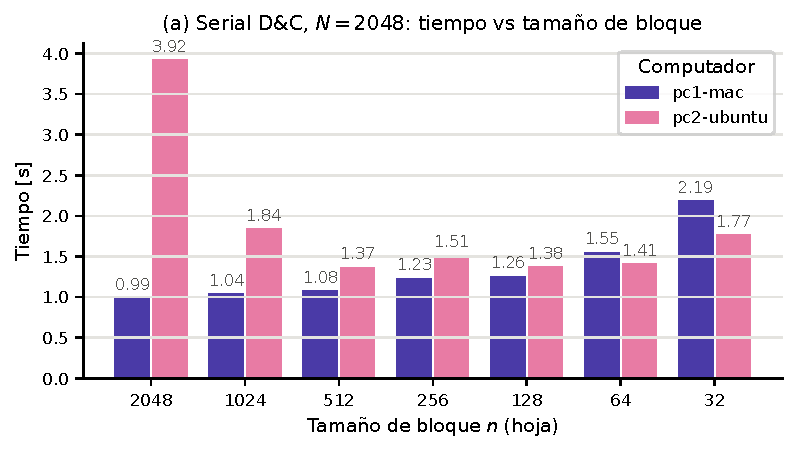
\includegraphics[width=0.8\linewidth]{a_serial_bloque.pdf}
  \caption{Tiempo de \texttt{serial.cpp} con $N=2048$ según el tamaño de hoja $n$.}
  \label{fig:a}
\end{figure}
\begin{table}[H]
\centering\small
\caption{Tiempo serial [s] para $N=2048$ según tamaño de bloque $n$ (mediana).}
\label{tab:a_serial_bloque}
\begin{tabular}{lll}
\toprule
 & pc1-mac & pc2-ubuntu \\
$n$ &  &  \\
\midrule
2048 & 0.988 & 3.923 \\
1024 & 1.045 & 1.842 \\
512 & 1.078 & 1.367 \\
256 & 1.233 & 1.514 \\
128 & 1.256 & 1.377 \\
64 & 1.552 & 1.411 \\
32 & 2.188 & 1.766 \\
\bottomrule
\end{tabular}
\end{table}

\nota{Observaciones (\pcA): el tiempo \emph{crece} monótonamente al achicar $n$: 0.99 s ($n=2048$), 1.04, 1.08, 1.23, 1.26, 1.55 y 2.19 s ($n=32$, $2.2\times$ más lento). En una sola hebra del M5, subdividir no conviene:
\begin{itemize}
\item La hoja i-k-j ya recorre $B$ y $C$ por filas (acceso contiguo, que el prefetcher de hardware anticipa bien y que se vectoriza con SIMD NEON). Además, la L2 del clúster de P-cores es grande (16 MB) y el ancho de banda de memoria es alto, así que la localidad extra del blocking aporta poco.
\item Overhead: con hojas de $n$ hay $(N/n)^3$ llamadas a \texttt{multiply\_leaf} (262\,144 con $n=32$, frente a 1 con $n=N$), y el loop interno tiene solo $n$ iteraciones (32 doubles = 2 líneas de caché de 128 B). Esto se traduce en más saltos, prólogo y epílogo de vectorización y peor prefetch.
\item Las tres submatrices de una hoja ocupan $3\cdot 8n^2$ B: 24 KB ($n=32$), 96 KB ($n=64$, cabe en L1D de 128 KB), 384 KB ($n=128$) y 1.5 MB ($n=256$). Aun cuando caben en L1/L2, la ganancia de localidad no compensa el overhead.
\item Lo importante es que este resultado es \emph{serial}. En paralelo, donde varios cores comparten la L2 y el ancho de banda, el blocking sí ayuda (ver (c) y (f)).
\item \textbf{Contraste con \pcB\ (Ryzen):} ahí el comportamiento es el \emph{opuesto} y muestra la clásica curva en U. Sin subdividir ($n=2048$) tarda 3.92 s; el óptimo está en $n=512$--$128$ (1.37--1.38 s), es decir, \textbf{2.9$\times$ más rápido}, y con $n=32$ vuelve a subir (1.77 s) por el overhead. En el Ryzen, $B$ (32 MB) no cabe en la L3 de 16 MB, la L2 es de solo 512 KB por core y el ancho de banda DDR4 es mucho menor, así que la versión sin bloques queda limitada por memoria (4.4 GFLOP/s con $N=2048$, frente a 12.8 GFLOP/s con $N=1024$, donde $B=8$ MB sí cabe en L3). El blocking mantiene los datos de la hoja en caché, lo que compensa con creces el overhead de la recursión. Conclusión: el mejor $n$ depende de la jerarquía de memoria de cada máquina.
\end{itemize}}

% ======================================================================
\section{(b) Algoritmo 1: paralelismo de datos con OpenMP}
\begin{lstlisting}[language=C++]
#pragma omp parallel for schedule(static)
for (int i = 0; i < N; ++i)
    for (int k = 0; k < N; ++k) {
        double a = A[i*N + k];
        for (int j = 0; j < N; ++j)
            C[i*N + j] += a * B[k*N + j];
    }
\end{lstlisting}
\nota{Implementación: se reparte el loop externo $i$ (filas de $C$) en bloques contiguos (\texttt{schedule(static)}). Cada thread escribe filas disjuntas de $C$, por lo que no hay carreras ni sincronización (solo la barrera implícita al final). El orden i-k-j recorre $B$ y $C$ por filas (acceso contiguo, vectorizable con SIMD). Como todas las iteraciones cuestan lo mismo, un scheduling estático es suficiente.}
\input{tablas/bcd_escalamiento_\pcA}
\nota{Observaciones Alg.~1 (\pcA, $N=2048$): $T(1)=0.99$ s y $T(8)=0.32$ s; $S=1.63,\,2.27,\,3.09$ y $E=0.82,\,0.57,\,0.39$ para $p=2,4,8$. El speedup está lejos del ideal:
\begin{itemize}
\item \textbf{Ancho de banda de memoria:} para cada fila $i$ se recorre toda $B$ (32 MB con $N=2048$, que no cabe en la L2 de 16 MB). Así, todos los threads compiten por leer $B$ desde DRAM y el kernel queda limitado por memoria, no por cómputo. Con $N=1024$ ($B=8$ MB cabe en L2) la eficiencia es claramente mejor (ver (f)).
\item \textbf{Cores heterogéneos:} el M5 tiene solo 4 P-cores. Con $p=8$, al menos 4 threads corren en E-cores (más lentos, con L2 propia de 6 MB). Probamos \texttt{schedule(dynamic,16)} y \texttt{guided}: solo mejoran $\sim$3--5\%, y usar $p=10$ casi no cambia el tiempo (0.29--0.31 s). Esto confirma que el límite principal es la memoria y no el desbalance.
\item No hay sincronización ni carreras (filas disjuntas), así que la pérdida no es por overhead de OpenMP.
\end{itemize}}

% ======================================================================
\section{(c) Algoritmo 2: dividir y conquistar con tareas OpenMP}
\begin{lstlisting}[language=C++]
void multiply_rec_task(A, B, C, n, depth) {
    if (C.size <= n) { multiply_leaf(A, B, C); return; }
    int h = C.size / 2;
    for (bi in {0,1}) for (bj in {0,1}) {
        #pragma omp task firstprivate(bi, bj) if(spawn)
        {   // C_ij += A_i1 B_1j ; luego C_ij += A_i2 B_2j  (en secuencia)
            multiply_rec_task(A(bi,0), B(0,bj), C(bi,bj), n, depth+1);
            multiply_rec_task(A(bi,1), B(1,bj), C(bi,bj), n, depth+1);
        }
    }
    #pragma omp taskwait
}
// main:  #pragma omp parallel  /  #pragma omp single  multiply_rec_task(...)
\end{lstlisting}
\nota{Detalles de implementación:
(1) Un solo thread (\texttt{single}) inicia la recursión dentro de una región \texttt{parallel} y el resto de los threads toma tareas del pool.
(2) En cada nivel se crean 4 tareas independientes, una por cuadrante $C_{ij}$. Los dos productos que acumulan en el mismo $C_{ij}$ se ejecutan en secuencia dentro de la misma tarea, así que dos tareas concurrentes nunca escriben el mismo bloque: no hay carreras, ni atomics, ni matrices temporales.
(3) \texttt{taskwait} garantiza que el bloque esté completo antes de retornar.
(4) Se usan vistas (\texttt{MatView}: puntero + stride) sin copiar datos, igual que en \texttt{serial.cpp}.
(5) Hay un cutoff opcional por profundidad (cláusula \texttt{if}). Con $n\ge 64$ no fue necesario, porque el número de tareas ya es moderado.
Número de tareas hoja: $(N/n)^2$ cuadrantes de $C$ (cada uno con $N/n$ productos secuenciales).}
\nota{Elección de $n=128$: se hizo un barrido de $n\in\{32,\dots,2048\}$ con $p=8$ (tabla y figura en (e)) y $n=128$ fue el más rápido para $N=2048$ (0.32 s) y también para $N=4096$ (2.4 s en una prueba preliminar). Justificación: (i) el bloque de trabajo de una hoja ($3\times128^2\times8$ B = 384 KB) cabe holgadamente en la L2 compartida, así que cada hoja reutiliza datos de caché en lugar de ir a DRAM; (ii) hay $(N/n)^2=256$ tareas sobre cuadrantes de $C$ (y 4096 hojas en total), mucho más que $p=8$, lo que permite balancear la carga entre P y E-cores; (iii) con $n\le64$ crece el overhead de recursión y de creación de tareas, y con $n\ge512$ hay muy pocas tareas (con $n=1024$ hay solo 4 cuadrantes, así que con $p=8$ quedan threads ociosos y el tiempo \emph{empeora}: 0.70 s).}
\input{tablas/e_alg2_bloques_\pcA}
\nota{Observaciones Alg.~2 (\pcA, $N=2048$, $n=128$): $T(1)=1.26$ s y $T(8)=0.32$ s; $S(8)=3.94$, $E(8)=0.49$. Es la versión que mejor escala. Su $T(1)$ es mayor que el del Alg.~1 (1.26 vs 0.99 s) por el overhead de la recursión, pero con $p=8$ alcanza el mismo tiempo absoluto y lo supera con $N=4096$ (2.96 vs 3.44 s). El blocking reduce el tráfico a memoria, que es justamente el cuello de botella del Alg.~1.}

% ======================================================================
\section{(d) Algoritmo 3: Numba}
\begin{lstlisting}[language=Python]
@njit(parallel=True, cache=True)
def matmul_prange(A, B, C):
    N = A.shape[0]
    for i in prange(N):
        for k in range(N):
            a = A[i, k]
            for j in range(N):
                C[i, j] += a * B[k, j]
\end{lstlisting}
\nota{Antes de medir se hace un warm-up (una llamada con una matriz de $8\times8$, que compila la función JIT para los mismos tipos) y otra llamada de warm-up tras cada \texttt{set\_num\_threads(p)}. Solo se mide la llamada al kernel. La verificación se hace con \texttt{np.allclose(C, A @ B)}.}
\nota{Observaciones Numba (\pcA, $N=2048$): $T(1)=1.08$ s (solo $\sim$8\% más lento que C++ \texttt{-O3}), $T(8)=0.32$ s, $S(8)=3.35$, $E(8)=0.42$. Con muy poco código se obtiene un rendimiento prácticamente igual al del Alg.~1 en C++, porque compila a LLVM igual que clang y el patrón de acceso es el mismo. Con $N=4096$ escala peor ($S(8)=2.2$ vs 2.5 en C++), posiblemente por la capa de threads por defecto en macOS (\texttt{workqueue}, sin afinidad ni control del scheduling). Ventaja: prototipado rápido. Desventaja: no permite paralelismo de tareas (Alg.~2) ni controlar el scheduling o la afinidad.}

% ======================================================================
\section{(e) Comparación y escalamiento}
\begin{figure}[H]\centering
  \includegraphics[width=\linewidth]{e_escalamiento_\pcA.pdf}
  \caption{$T(p)$, $S(p)$ y $E(p)$ de las tres versiones con $N=2048$ en \pcA. La línea punteada es la curva ideal.}
\end{figure}
\nota{Elección de $T(1)$: se usa el tiempo de \emph{la misma versión} ejecutada con 1 thread (speedup relativo). Así se aísla la escalabilidad de la paralelización y no se mezclan diferencias de implementación serial (por ejemplo, el overhead de la recursión en el Alg. 2 o el JIT en Numba). Para ser transparentes, la tabla incluye también $S_{abs}$ respecto al mejor tiempo serial medido.}
\begin{figure}[H]\centering
  \includegraphics[width=\linewidth]{e_alg2_bloques_\pcA.pdf}
  \caption{Algoritmo 2 con distintos tamaños de bloque $n$, $N=2048$, \pcA.}
\end{figure}
\nota{Observaciones (e):
\begin{itemize}
\item Ninguna versión se acerca al ideal: $E(8)$ entre 0.39 y 0.49 con $N=2048$. Las tres versiones comparten el mismo patrón (buena eficiencia con $p=2$ y caída con $p=4$ y 8), lo que apunta a una limitación del hardware (memoria compartida y cores heterogéneos) más que a la implementación.
\item Orden de escalabilidad: Alg.~2 $>$ Numba $\gtrsim$ Alg.~1.
\item Efecto de $n$ en el Alg.~2: $n=2048$ no tiene tareas, así que $S\approx1$; $n=1024$ tiene solo 4 tareas, por lo que $S(8)<S(4)$. Para $n\le256$ el speedup con $p=8$ está entre 3.2 y 4.6. Los $n$ chicos (32, 64) tienen el mejor $S$ \emph{relativo} (4.2--4.6), porque su $T(1)$ es muy malo, pero en tiempo absoluto pierden contra $n=128$. Esto muestra por qué el speedup relativo debe leerse junto al tiempo absoluto.
\end{itemize}}

% ======================================================================
\section{(f) Escalabilidad débil}
\nota{Definición: con $N$ fijo, $E(p)=T(1)/(p\,T(p))$ es la eficiencia fuerte. Para escalabilidad débil el trabajo por thread debe ser constante, pero como $W\propto N^3$, los $N$ pedidos no permiten mantener $W/p$ exacto (solo $1024\to p{=}1$ y $2048\to p{=}8$). Se define entonces la eficiencia normalizada por trabajo
$E_w(N,p)=\dfrac{(N/N_0)^3\,T(N_0,1)}{p\,T(N,p)}$ con $N_0=1024$, que compara el rendimiento por thread (FLOP/s/thread) con el caso base serial. $E_w=1$ significa que cada thread rinde lo mismo que un thread solo con el problema chico.}
\begin{figure}[H]\centering
  \includegraphics[width=\linewidth]{f_escalabilidad_\pcA.pdf}
  \caption{Arriba: eficiencia fuerte $E(p)$ para cada $N$. Abajo: eficiencia débil $E_w(N,p)$. \pcA.}
\end{figure}
\nota{Observaciones (f): \textbf{el desempeño paralelo no se mantiene al crecer $N$}.
\begin{itemize}
\item $E_w(N,8)$: Alg.~1 $0.52\to0.37\to0.28$; Alg.~2 $0.54\to0.46\to0.40$; Numba $0.53\to0.40\to0.26$ para $N=1024\to2048\to4096$.
\item Explicación: el tamaño de $B$ es 8 MB, 32 MB y 128 MB. Solo con $N=1024$ cabe en la L2 de 16 MB, así que con $N$ mayor las versiones de paralelismo de datos quedan limitadas por el ancho de banda de DRAM, que no crece con $p$.
\item El Alg.~2 es el que mejor resiste el aumento de $N$, porque sus hojas de 128$\times$128 trabajan en caché independientemente de $N$. Con $N=4096$ y $p=8$ es el más rápido (2.96 s vs 3.44 s del Alg.~1 y 4.01 s de Numba).
\item \textbf{En \pcB\ el efecto es mucho más fuerte}: $E_w(N,8)$ del Alg.~1 cae $0.55\to0.19\to0.12$ y el de Numba $0.48\to0.17\to0.11$, porque al pasar de $N=1024$ a 2048 la matriz $B$ deja de caber en la L3 (el rendimiento serial cae de 12.8 a 4.4 GFLOP/s). En cambio, el Alg.~2 \emph{mantiene e incluso mejora} su eficiencia débil ($0.49\to0.50\to0.57$) y su rendimiento con $p=8$ crece de 46 a 54 GFLOP/s. Con $N=4096$ y $p=8$ el Alg.~2 es 4.5$\times$ más rápido que el Alg.~1 (2.55 s vs 11.58 s). Este es el resultado más claro del trabajo: la escalabilidad débil depende de que el working set de cada thread quepa en caché, y eso es justamente lo que garantiza el blocking.
\item También baja $E_w(N,1)$ (por ejemplo 0.87 para el Alg.~1 con $N=4096$): incluso en serial el rendimiento por FLOP empeora con $N$, por el mismo efecto de caché.
\end{itemize}}

% ======================================================================
\section{(g) Segundo computador}
\begin{figure}[H]\centering
  \includegraphics[width=\linewidth]{e_escalamiento_\pcB.pdf}
  \caption{$T(p)$, $S(p)$ y $E(p)$ con $N=2048$ en \pcB.}
\end{figure}
\input{tablas/bcd_escalamiento_\pcB}
\begin{figure}[H]\centering
  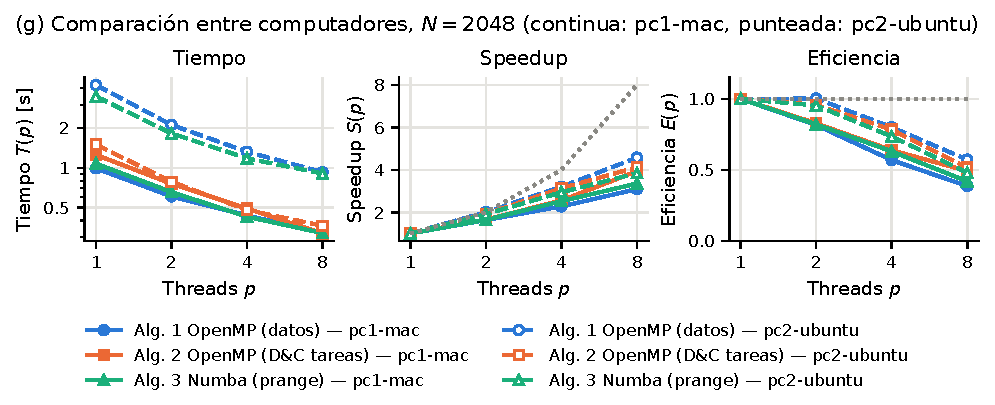
\includegraphics[width=\linewidth]{g_comparacion.pdf}
  \caption{Comparación de ambos computadores con $N=2048$ (Alg.~2 con $n=128$). Línea continua y marcadores rellenos: \pcA; línea punteada y marcadores vacíos: \pcB.}
\end{figure}
\begin{figure}[H]\centering
  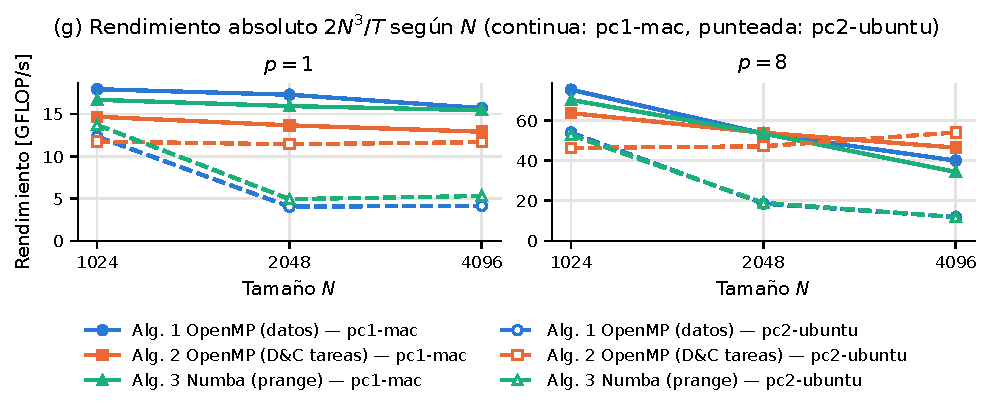
\includegraphics[width=\linewidth]{g_gflops.pdf}
  \caption{Rendimiento absoluto (GFLOP/s) según $N$ con $p=1$ y $p=8$ en ambos computadores (Alg.~2 con $n=128$).}
\end{figure}
\begin{figure}[H]\centering
  \includegraphics[width=\linewidth]{e_alg2_bloques_\pcB.pdf}\\[4pt]
  \includegraphics[width=\linewidth]{f_escalabilidad_\pcB.pdf}
  \caption{Algoritmo 2 según $n$ y escalabilidad según $N$ en \pcB.}
\end{figure}
\nota{Observaciones (g). Correctitud: las tres versiones entregan el mismo checksum en ambas máquinas (error máximo $=0$ frente a la referencia), lo que confirma la inicialización determinista.
\begin{itemize}
\item \textbf{Tiempo serial:} el M5 es 4$\times$ más rápido en el problema base ($n=N$): 0.99 s frente a 3.92 s con $N=2048$. La diferencia no se explica por la frecuencia (del mismo orden en ambas) sino por la memoria. El M5 tiene una L2 de 16 MB y memoria unificada LPDDR5X de gran ancho de banda, mientras que el Ryzen usa DDR4 de doble canal. Además, el M5 mantiene $\sim$16--18 GFLOP/s para todo $N$, mientras que el Ryzen cae de 12.8 a $\sim$4 GFLOP/s cuando $B$ deja de caber en L3. Con blocking (\texttt{serial.cpp} con $n=128$) la diferencia se reduce a 1.26 frente a 1.38 s.
\item \textbf{Speedup:} en el Ryzen, el Alg.~1 tiene \emph{mejor} speedup relativo ($S(8)=4.58$ frente a 3.09 con $N=2048$), pero su tiempo absoluto es 2.9$\times$ peor (0.93 frente a 0.32 s). Su $T(1)$ es tan lento (está limitado por la latencia de memoria) que más threads ayudan a tener más accesos en vuelo. Esto muestra por qué el speedup relativo debe leerse junto al tiempo absoluto.
\item \textbf{Límite de memoria:} con $N=4096$, el Alg.~1 y Numba en el Ryzen no mejoran de $p=4$ a $p=8$ (11.5 $\to$ 11.6 s y 11.2 $\to$ 11.6 s): el ancho de banda DDR4 queda saturado con 4 threads. El Alg.~2 sí sigue escalando ($S(8)=4.62$) y con $p=8$ alcanza 54 GFLOP/s, \emph{superando} al M5 (46 GFLOP/s) en la misma configuración.
\item \textbf{Cores y SMT:} el Ryzen tiene 6 cores físicos homogéneos con SMT. Con $p=8$, 2 cores ejecutan 2 hilos cada uno y comparten FPU, L1 y L2, por lo que de $p=4$ a $p=8$ la ganancia es sublineal. El M5 tiene 10 cores físicos sin SMT, pero solo 4 son P-cores; con $p=8$ al menos 4 threads corren en E-cores más lentos. En ambos casos, $p=8$ no equivale a 8 cores iguales.
\item \textbf{Elección de $n$:} en el Ryzen, el barrido con $p=8$ da $n=64$, 128 y 256 prácticamente empatados (0.35--0.36 s, dentro del ruido). $n=128$ es razonable en ambas máquinas: $3\times128^2\times8$ B = 384 KB cabe en la L2 de 512 KB de un core Zen 2 y en la L2 del M5.
\item \textbf{Anomalías:} con $n=2048$ (sin tareas) el tiempo del Alg.~2 en el Ryzen \emph{aumenta} con $p$ (3.54 a 4.05 s). Una hipótesis es que los threads ociosos hacen busy-wait (libgomp) en la barrera y reducen la frecuencia boost del core que trabaja. Con $n=1024$ y $p=2$ no hay ganancia (1.92 frente a 1.89 s): las 4 tareas leen cuadrantes distintos de $B$ de 8 MB cada uno y saturan la memoria, a diferencia del Alg.~1, donde los threads comparten las mismas filas de $B$ en caché.
\item \textbf{Numba vs C++:} en el Ryzen, Numba es incluso más rápido que g++ con 1 thread (3.48 frente a 4.24 s con $N=2048$). Ambos compiladores generan código distinto (LLVM frente a GCC), pero los dos quedan limitados por memoria.
\item \textbf{Ruido:} el PC2 corre bajo WSL2, y algunas mediciones tienen más variabilidad (por ejemplo Numba con $N=1024$ y $p=2$). Por eso se reporta la mediana.
\end{itemize}}

% ======================================================================
\section{Conclusiones}
\nota{(1) El problema base en C++ escala hasta $S\approx3$ con 8 threads en el M5, limitado por memoria. (2) Dividir y conquistar tiene peor tiempo serial, pero escala mejor y es más robusto al crecer $N$ gracias a la localidad de caché; $n$ es un compromiso entre overhead de tareas y paralelismo disponible. (3) Numba logra un rendimiento cercano a C++ con mínimo esfuerzo, pero con menos control. (4) Entre máquinas, la jerarquía de memoria domina más que la frecuencia o el número de cores: en el M5 (L2 grande y alto ancho de banda) la versión simple ya es eficiente, mientras que en el Ryzen el blocking es indispensable (2.9$\times$ en serial y 4.5$\times$ con $N=4096$, $p=8$). (5) La escalabilidad débil solo se mantiene en el Alg.~2, cuyo working set por tarea es independiente de $N$.}

% ======================================================================
\section*{Declaración de uso de IA}
Para este trabajo se usó Claude (Anthropic) mediante Claude Code como asistente para: escribir el código de las versiones paralelas, los scripts de benchmarking y de gráficos, y un borrador inicial de la estructura del informe con observaciones sobre los resultados. Todo el código fue revisado y ejecutado por el grupo, los resultados corresponden a mediciones reales en nuestros computadores, y el análisis y la redacción final son de los integrantes.
\nota{Ajustar según cómo lo usaron realmente.}

\appendix
\section{Tablas completas}
\input{tablas/f_escalabilidad_\pcA}
\input{tablas/e_alg2_bloques_\pcB}
\input{tablas/f_escalabilidad_\pcB}

\end{document}
